%
% achr.tex -- Achromat
%
% (c) 2018 Prof Dr Andreas Müller, Hochschule Rapperswil
%
\documentclass[tikz,12pt]{standalone}
\usepackage{times}
\usepackage{amsmath}
\usepackage{txfonts}
\usepackage[utf8]{inputenc}
\usepackage{graphics}
\usepackage{color}
\usepackage{pifont}
\usetikzlibrary{arrows,intersections,math,calc}
\begin{document}

\def\punkt#1{
        \fill[color=white] #1 circle[radius=0.08];
        \draw #1 circle[radius=0.08];
}

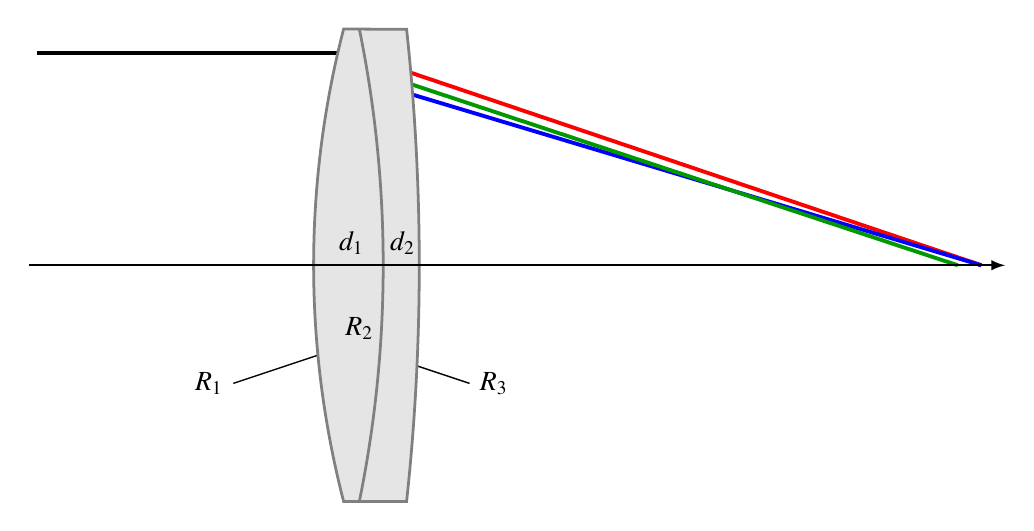
\begin{tikzpicture}[>=latex,thick]

\def\done{-0.1}
\def\dtwo{0.1}
\def\dthree{0.7}

\def\Rone{12}
\def\Rtwo{15}
\def\Rthree{28}

\def\h{3}

\pgfmathparse{3/\Rone}
\xdef\x{\pgfmathresult}
\pgfmathparse{atan(\x/sqrt(1-\x*\x))}
\xdef\aone{\pgfmathresult}

\pgfmathparse{3/\Rtwo}
\xdef\x{\pgfmathresult}
\pgfmathparse{atan(\x/sqrt(1-\x*\x))}
\xdef\atwo{\pgfmathresult}

\pgfmathparse{3/\Rthree}
\xdef\x{\pgfmathresult}
\pgfmathparse{atan(\x/sqrt(1-\x*\x))}
\xdef\athree{\pgfmathresult}

\definecolor{darkgreen}{rgb}{0,0.6,0}

\draw[line width=1.4pt,color=red] (0,2.7)--(8,0);
\draw[line width=1.4pt,color=blue] (0,2.4)--(8,0);
\draw[line width=1.4pt,color=darkgreen] (0,2.55)--(7.7,0);

\draw[line width=1.4pt,color=black] (-4,2.7)--(0,2.7);

\node at (-1.5,-1.5) [left] {$R_1$};
\node at (1.5,-1.5) [right] {$R_3$};

\draw[line width=0.5pt] (-1.5,-1.5)--(0,-1);
\draw[line width=0.5pt] (1.5,-1.5)--(0,-1);

\fill[color=gray!20]
	({\done},{\h}) arc (180-\aone:180+\aone:\Rone)
	--
	({\dthree},{-\h}) arc (-\athree:\athree:\Rthree)--cycle;

\draw[line width=1pt,color=gray]
	({\done},{\h}) arc (180-\aone:180+\aone:\Rone)
	--
	({\dthree},{-\h}) arc (-\athree:\athree:\Rthree)--cycle;
\draw[line width=1pt,color=gray]
	({\dtwo},{\h}) arc (\atwo:-\atwo:\Rtwo);
%\draw[color=gray]
%	({\dthree},{\h}) arc (\athree:-\athree:\Rthree);

\node at (0.1,-0.8) {$R_2$};

\node at (0,0) [above] {$d_1$};
\node at ({\dthree-0.05},0) [above] {$d_2$};

\draw[->,line width=0.7pt] (-4.1,0)--(8.3,0);

\punkt{(8,0)}
\punkt{(7.7,0)}

\end{tikzpicture}

\end{document}

